\section{Experiment} In this section, We conduct experiments to evaluate \our, focusing on two key objectives: to validate our framework's ability to generate diverse, controllable, and challenging scenarios, and to demonstrate the effectiveness of our core components: the two-stage VLM planner and the gradient-free guidance mechanism. All experiments are conducted on the Argoverse 2 dataset~\citep{wilson2023argoverse}.We leverage these real-world recordings as a foundation to generate scenarios enriched with complex social interactions.

We evaluate performance using key interaction metrics. To evaluate the quality of generated scenarios, we compute Engagement Ratio.  The Engagement Ratio is calculated by setting a threshold for Time-to-Collision (TTC), defined as the estimated time until a collision between vehicles based on their current trajectories and speeds. Scenarios with a maximum TTC exceeding this threshold are classified as engagement scenarios. We also measure the maximum relative velocity between vehicles to quantify interaction intensity. Furthermore, we compute the maximum acceleration to capture the aggressiveness and non-cooperative nature of the driving behaviors. To evaluate task completion, we report the Extrinsic Reward regarding the vehicle's trajectory, which reflects the specific driving objectives.


\begin{figure}[htbp]
    \centering
    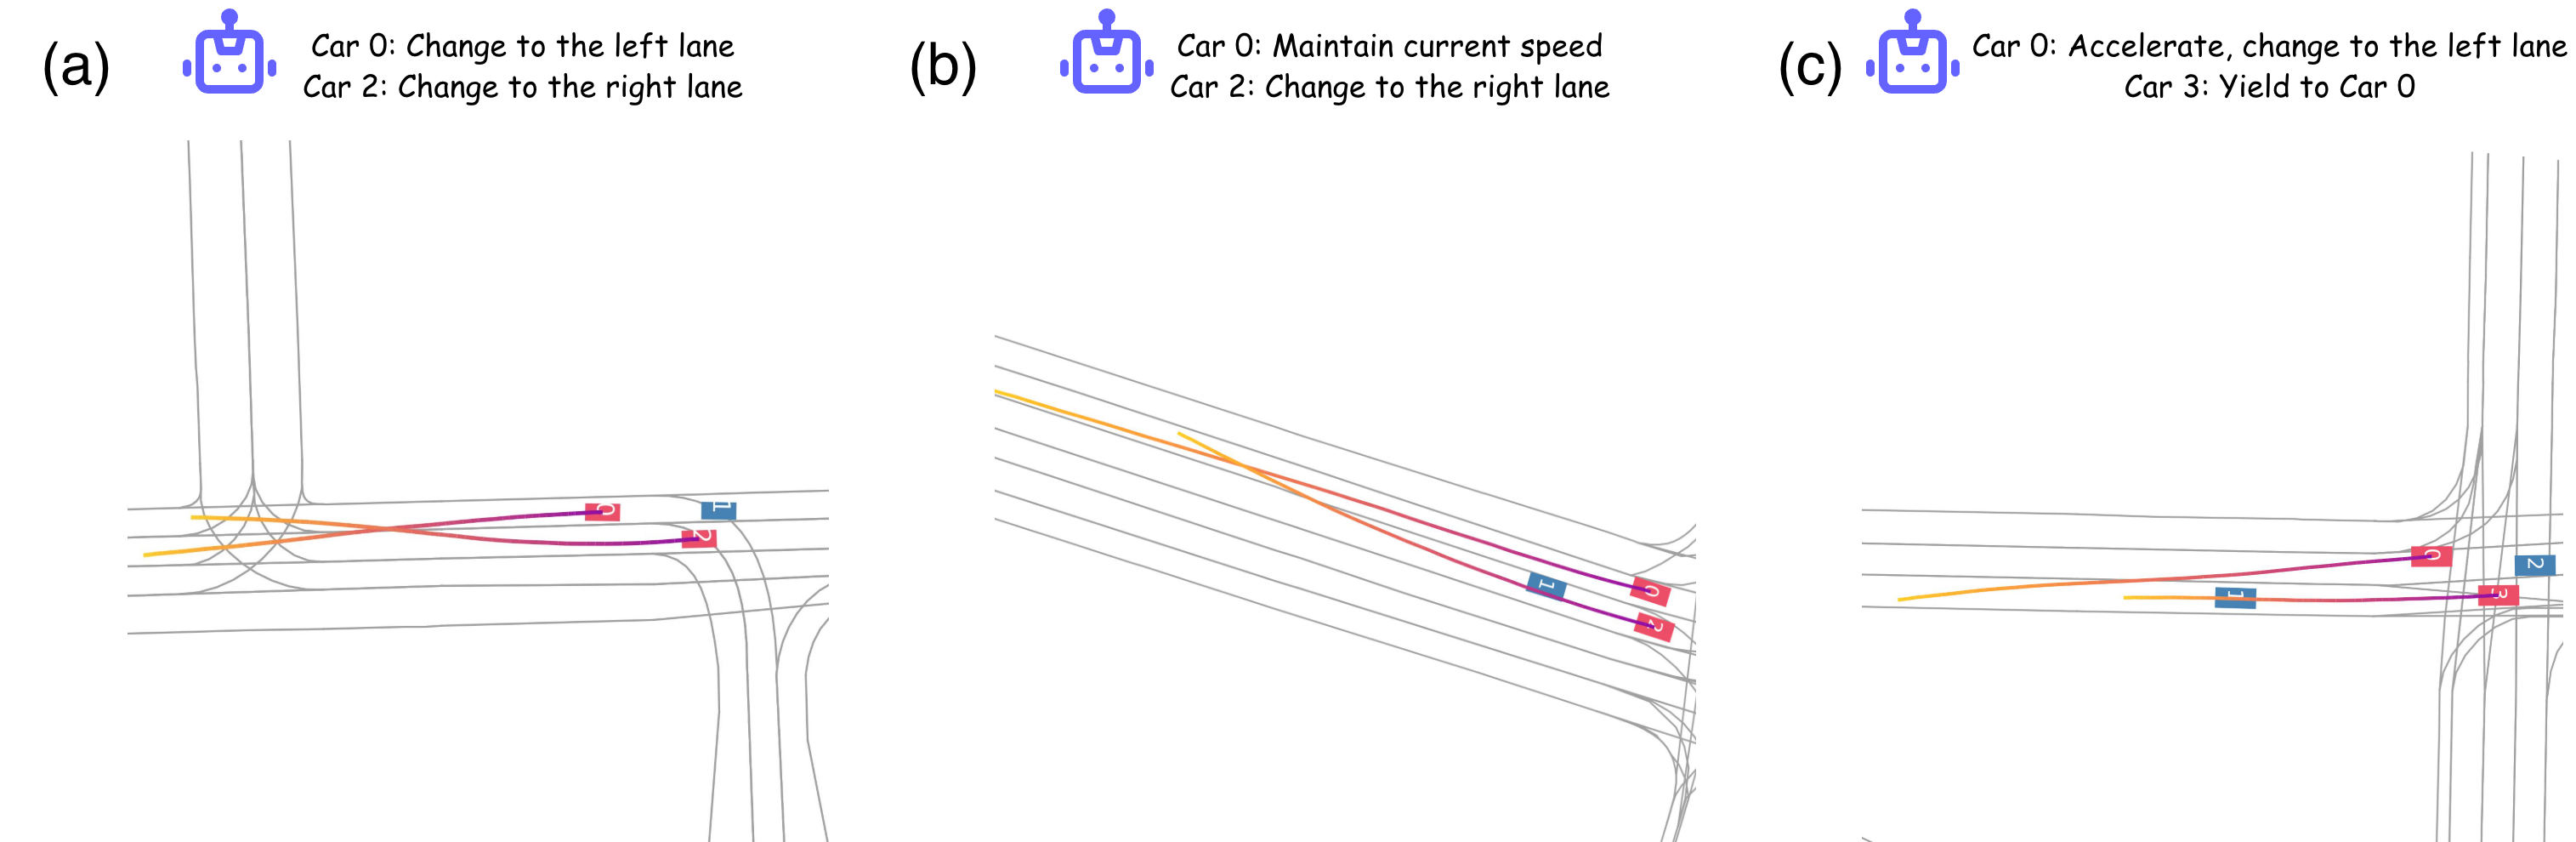
\includegraphics[width=1.0\textwidth]{figures/changan_exp.drawio.png}
    \caption{Results of interactive scenarios generated by \our. Our framework translates high-level VLM proposals into diverse, social interactive trajectories. Red vehicles correspond to the pair selected by the VLM for interaction.}
    \label{fig:socialdrivegen-example}
\end{figure}

\subsection{Qualitative Analysis: Interactive Scenario Generation}

Figure~\ref{fig:socialdrivegen-example} provides a qualitative analysis of scenarios generated by \our. Each subplot visualizes the trajectories of two interacting vehicles selected by the VLM, generated in response to high-level adversarial proposals. As illustrated, the generated trajectories are physically plausible, maintaining kinematic smoothness and collision-free states. Crucially, the results highlight the diversity of our framework, which successfully synthesizes a wide spectrum of driving behaviors—ranging from cooperative merging to competitive gaming.

Specifically, in Figure~\ref{fig:socialdrivegen-example}(a), both Car 0 and Car 2 attempt a concurrent lane change, resulting in a coordinated cooperative maneuver. In Figure~\ref{fig:socialdrivegen-example}(b), a non-cooperative scenario is synthesized where Car 0 maintains its speed and refuses to yield to the merging Car 2. In Figure~\ref{fig:socialdrivegen-example}(c), Car 3 exhibits yielding behavior, decelerating to accommodate Car 0’s lane change intent. Collectively, these examples demonstrate our framework's capability to translate high-level VLM proposals into concrete scenarios characterized by enhanced interaction intensity.

\subsection{Component Analysis and Ablation Study}

To validate the individual contributions of our core modules, we conduct an ablation study focusing on two critical aspects: the decision-making capability of the VLM planner and the optimization efficiency of the diffusion guidance mechanism. Table~\ref{tab:ablation_study} summarizes the performance in terms of Engagement Ratio and kinematic dynamics (Relative Velocity and Acceleration).

\begin{table}[ht]
\centering
\renewcommand{\arraystretch}{1.1}
\caption{Ablation Study on the Components of \our. We evaluate the contribution of the two stage VLM-based proposal generation and the stepwise guidance mechanism.}
\label{tab:ablation_study}
\setlength{\tabcolsep}{0pt}
\begin{tabular}{lccc}
\toprule
\textbf{Method} & 
\parbox[c]{3cm}{\centering \textbf{Engagement \\ Ratio }\\ ($\text{TTC} < 4.0$s)} & 
\parbox[c]{2.25cm}{\centering \textbf{Relative \\ Velocity \\ ($m/s$)}} & 
\parbox[c]{2.25cm}{\centering \textbf{ Acceleration \\ ($m/s^2$)}} \\
\midrule

% \multicolumn{4}{@{}l}{\textit{VLM Proposal/Stage Ablation}} \\
 Random Proposal  & 34.55 & 3.01 & 6.50 \\
 Single Stage VLM & 50.91 & 3.65 & 7.25 \\
\midrule

% \multicolumn{4}{@{}l}{\textit{Diffusion Guidance Ablation}} \\
    Diffusion-ES~\citep{yang2024diffusion} & 60.00 & 4.10 & 7.85 \\
\midrule

    \textbf{Ours (Full)} & \textbf{67.27} & \textbf{4.32} & \textbf{8.11} \\
\bottomrule
\end{tabular}
\end{table}

\paragraph{Effectiveness of the Two-Stage VLM Planner}

We first investigate the necessity of our hierarchical planning strategy by comparing it against two baselines: (1) \textit{Random Proposal}, which assigns pre-defined actions stochastically, and (2) \textit{Single-Stage VLM}, which attempts to generate proposals directly from the initial scene without intermediate reasoning.

As shown in Table~\ref{tab:ablation_study}, \our achieves an Engagement Ratio of $67.27\%$, surpassing the Single-Stage ($50.91\%$) and Random ($34.55\%$) methods by significant margins. The poor performance of the Random baseline highlights that high-stakes interactions are rare and require intelligent initiation. More importantly, the 16.36\% performance gap between our method and the Single-Stage VLM validates our hierarchical design philosophy. Complex traffic scenarios involve subtle dynamic cues that are difficult to capture via a direct mapping from raw states to proposals. By decomposing the task into a ``Describe-then-Propose'' pipeline, our framework mimics a Chain-of-Thought reasoning process. The first stage forces the model to explicitly articulate the global context and social intentions into a semantic description $D_{\text{scene}}$. This intermediate reasoning step serves as a critical grounding signal, enabling the second stage to strategically select the most relevant vehicle pair and formulate precise adversarial goals that are deeply contextualized rather than visually reactive.

\paragraph{Effectiveness of Iterative Guidance}

Second, we evaluate the impact of our gradient-free guidance mechanism. We compare our step-wise approach against \textit{Diffusion-ES}~\citep{yang2024diffusion}, a baseline that applies reward-based guidance only at the terminal step of the denoising process.

The results demonstrate that \our outperforms the baseline in both interaction success (higher Engagement Ratio) and dynamic intensity (higher Relative Velocity and Acceleration). We attribute this to the fundamental difference in optimization timing. The diffusion process generates trajectories by progressively refining noise; applying guidance only at the final step is often ``too late'' to significantly alter the trajectory's topological structure or correct early-stage deviations. in contrast, our iterative guidance actively optimizes the population distribution at each denoising step. This allows the model to correct the trajectory manifold early in the generation process, effectively steering the agents toward higher-reward solutions. Consequently, \our is capable of generating scenarios that are not only compliant with the proposal but also exhibit the challenging dynamics and high speeds required for robust safety testing.

% \subsection{Examples Analysis and Controllability}

% Furthermore, This visual diversity is a direct result of our social-aware reward function. By design, the framework's controllability is governed by the social-aware parameters $\lambda$ and $\phi$. Adjusting these weights allows \our to influence the resulting driving dynamics.

\subsection{Controllability via Social Preferences}

To analyze the behavioral trade-offs induced by different social parameters, we shift our focus to the balance between interaction intensity and task performance. We report Engagement Ratio, Acceleration, and specifically the Extrinsic Reward, as the latter directly reflects the agent's adherence to navigational goals when social weights vary. Our proposed reward decomposition in Eq.~\eqref{eq:social_reward} introduces two interpretable control knobs: the \textbf{social orientation angle} $\phi$, which governs the agent's interaction style (e.g., aggressive vs. prosocial), and the \textbf{intrinsic reward magnitude} $\lambda$, which regulates the trade-off between social compliance (safety/comfort) and task completion (extrinsic goals). We set a rational egoist ($\lambda=1, \phi=0$) as the baseline. To demonstrate the controllability of our framework, we configure surrounding social vehicles as rational egoists to simulate a standard traffic environment.

\begin{table}[ht]
\centering
\renewcommand{\arraystretch}{1.1}
\caption{Quantitative comparison of generated trajectories under varying social preference parameters ($\lambda, \phi$), demonstrating their impact on interaction intensity, acceleration, and task performance.}
\label{tab:social_exp}
\setlength{\tabcolsep}{0pt}
\begin{tabular}{lccc}
\toprule
\parbox[c]{3.25cm}{\textbf{Social \\ Preference}} & 
\parbox[c]{3cm}{\centering \textbf{Engagement \\ Ratio }\\ ($\text{TTC} < 4.0$s)} & 
\parbox[c]{3cm}{\centering \textbf{Acceleration \\ ($m/s^2$)}} & 
\parbox[c]{3cm}{\centering \textbf{ Extrinsic \\ Reward}} \\
\midrule

% \multicolumn{4}{@{}l}{\textit{VLM Proposal/Stage Ablation}} \\
$\lambda = 1.0, \phi = 0$  & 67.27 & 8.11 & 0.37 \\
\midrule
% $\lambda = 1.0, \bm{\phi = \frac{\pi}{4}}$ & 63.64 & 7.97 & 0.48 \\
% % \multicolumn{4}{@{}l}{\textit{Diffusion Guidance Ablation}} \\
% $\lambda = 1.0, \bm{\phi = -\frac{\pi}{4}}$ & 72.73 & 8.16 & 0.31 \\
% $\bm{\lambda = 0.5}, \phi = 0$ & TBD & TBD & TBD \\
% $\bm{\lambda = 0.3}, \phi = 0$ & 69.09 & 8.28 & 0.69 \\
$\lambda = 1.0, \bm{\phi = \frac{\pi}{4}}$ & 63.64 (\textcolor{softblue}{-5.40\%}) & 7.97 (\textcolor{softblue}{-1.73\%}) & 0.48 (\textcolor{softred}{+29.73\%}) \\
$\lambda = 1.0, \bm{\phi = -\frac{\pi}{4}}$ & 72.73 (\textcolor{softred}{+8.12\%}) & 8.16 (\textcolor{softred}{+0.62\%}) & 0.31 (\textcolor{softblue}{-16.22\%}) \\
$\bm{\lambda = 0.5}, \phi = 0$ & 65.45 (\textcolor{softblue}{-2.71\%}) & 8.17 (\textcolor{softred}{+0.74\%}) & 0.60 (\textcolor{softred}{+62.16\%}) \\
$\bm{\lambda = 0.3}, \phi = 0$ & 69.09 (\textcolor{softred}{+2.71\%}) & 8.28 (\textcolor{softred}{+2.10\%}) & 0.69 (\textcolor{softred}{+86.49\%}) \\
\bottomrule
\end{tabular}
\end{table}


\paragraph{Impact of Social Orientation ($\phi$)}

We first examine how the directional preference $\phi$ influences the style of interaction. By modulating $\phi$ with fixed $\lambda$, we effectively shift the agent's behavior along the SVO spectrum without altering its high-level goal. As shown in Table~\ref{tab:social_exp}, setting $\phi = -\frac{\pi}{4}$ (representing a competitive or adversarial persona) leads to an $8.12\%$ increase in Engagement Ratio compared to the baseline ($\phi=0$). This suggests that negative angular preferences encourage the agent to prioritize its own intrinsic utility over the opponent's, resulting in more assertive behaviors such as forcing a merge or refusing to yield, thereby intensifying the interaction. Conversely, a prosocial setting ($\phi = \frac{\pi}{4}$) reduces the Engagement Ratio by $5.40\%$, as the agent actively seeks to minimize the opponent's discomfort, often yielding early to avoid high-stakes scenarios. This validates that $\phi$ serves as an effective parameter for controlling the ``aggressiveness'' of the generated scenarios.

\paragraph{Impact of Intrinsic Magnitude ($\lambda$)}

Next, we evaluate the role of $\lambda$ in balancing social constraints against task objectives. In our framework, a high $\lambda$ implies a socially compliant driver who strictly adheres to safety and comfort norms, potentially at the cost of task efficiency. As we progressively decrease $\lambda$ from $1.0$ to $0.3$, the agent becomes increasingly goal-oriented and egoistic, reducing the weight of social penalties. The results in Table~\ref{tab:social_exp} reveal a dramatic monotonic increase in Extrinsic Reward, peaking at $+86.49\%$ for $\lambda=0.3$. This indicates that as social constraints are relaxed, the agent becomes more efficient at achieving the VLM-specified objectives (e.g., reaching a target lane quickly), even if it requires more dynamic maneuvers. Notably, the Engagement Ratio remains high ($69.09\%$) at lower $\lambda$, confirming that the agent maintains interactivity but changes its motivation: from ``interacting carefully'' to ``interacting efficiently''. This validates our decomposition strategy, proving that we can disentangle extrinsic task motivations from intrinsic social constraints to generate diverse driving profiles.


% \begin{table*}[ht]
%     \renewcommand{\arraystretch}{1.2}
%     \caption{Ablation Study on the Components of \our. We evaluate the contribution of the two stage VLM-based proposal and the iterative guidance mechanism.}
%     \small
%     \label{tab:ablation_study_socialdrivegen}
%     \centering
%     \begin{tabular}{l c c c c}
%         \toprule
%         \textbf{Method} & Engagement Ratio (\%) & Relative Velocity & Max Acceleration & Mean Acceleration \\
%         & ($\text{TTC} < 4.0\text{s}$) & ($\text{m/s}$) & ($\text{m/s}^2$) & ($\text{m/s}^2$) \\
%         \midrule
%         \multicolumn{5}{@{}l}{\textit{VLM Proposal/Stage Ablation}} \\
%         \quad Random Proposal & $34.55$ & $3.01$ & $6.50$ & $1.65$ \\
%         \quad Single Stage VLM & $50.91$ & $3.65$ & $7.25$ & $1.90$ \\
%         \midrule
%         \multicolumn{5}{@{}l}{\textit{Diffusion Guidance Ablation}} \\
%         \quad Vanilla Evolutionary Guidance & $60.00$ & $4.10$ & $7.85$ & $2.15$ \\
%         \bottomrule
%         \noalign{\smallskip}
%         \textbf{Ours (Full)} & $\mathbf{67.27}$ & $\mathbf{4.32}$ & $\mathbf{8.11}$ & $\mathbf{2.19}$ \\
%         \noalign{\smallskip}
%         \toprule
%     \end{tabular}
% \end{table*}

% \begin{enumerate} 
% \item How does each component of our framework contribute to the overall performance?
% \item Can our framework generate diverse and challenging game-theoretic scenarios?
% \item Can the generated scenarios be effectively used to improve the performance of downstream driving policies? 
% \end{enumerate}

% \subsection{Dataset} We conduct our experiments using the Argoverse 2 dataset, a widely-used and large-scale dataset for trajectory prediction. This dataset is well-suited for our purposes due to its extensive observation window of 5 seconds and a long prediction horizon of 6 seconds, which provides sufficient context and foresight for complex social interactions.

% \subsection{Framework Component Ablation} 

% To validate the effectiveness and synergistic effects of each component within our framework, we conduct a comprehensive ablation study. This section is structured to demonstrate the significane of our two-stage VLM-based planner and the efficiency of our iterative guidance mechanism in generating diverse and challenging scenarios.

% \subsubsection{Ablation of the VLM-based Planner} We compare our two-stage VLM-based planner against the following baselines: \begin{itemize} \item \textbf{Random Proposal}: This method randomly selects a pair of vehicles and assigns them a set of pre-defined adversarial actions (e.g., accelerate, decelerate, lane change). This baseline represents a simple, non-intelligent approach to scenario generation. \item \textbf{Single-stage VLM}: We implement the method that the VLM is instructed to directly generate a complete, executable reward function from the initial scenario state.  \end{itemize}

% \paragraph{Metrics} To measure the diversity and adversarial nature of the generated scenarios, we employ three key quantitative metrics that capture different aspects of vehicle dynamics. We calculate \textbf{Time-to-Collision (TTC)}, where a lower value indicates a higher risk and more adversarial scenario. We also measure \textbf{Relative Velocity} to quantify the intensity of interactions and \textbf{Acceleration} to capture the aggression and non-cooperative nature of the driving behaviors.

% % \textbf{Results and Analysis}
% % TODO


% \subsubsection{Ablation of the Diffusion Guidance} To validate the efficiency and effectiveness of our iterative reward-guided sampling, we compare our approach against a baseline that performs guidance only on the final denoised samples.

% \paragraph{Experiment Setup} We compare our approach against the \textbf{End-of-Process Guidance Baseline}, which follows the guided method in Diffusion-ES \cite{yang2024diffusion}. This baseline runs a full reverse diffusion process to obtain a population of clean trajectories, and applies the reward function only to these final trajectories for scoring and selection, without any intermediate guidance. In contrast, our \textbf{Iterative Guidance (Our Method)}, as presented in Algorithm \ref{alg:denoise_sample}, performs reward-based sampling at each step of the reverse diffusion process to progressively guide the population toward high-reward trajectories, thereby enhancing efficiency.

% \paragraph{Metrics} In addition to evaluating the generation quality of all baseline and proposed methods, we also monitor the convergence speed to validate the effectiveness of the diffusion guidance component. We track \textbf{Convergence Speed} by plotting the average reward of the population as a function of the number of search steps, hypothesizing that our method will converge faster. We also compare \textbf{Final Reward}, expecting our method to achieve a higher maximum and average reward after a fixed number of iterations. Finally, we evaluate \textbf{Reward per Sample} to measure efficiency by comparing the number of diffusion model calls required to reach a certain reward threshold, anticipating our method to be more sample-efficient.


% \subsection{Diversity and Controllability of Generated Scenarios}

%  To validate the ability of our framework to generate a diverse spectrum of driving behaviors, we assess the controllability of our social-aware reward function. The objective of this experiment is to demonstrate that by adjusting the weights of egoism and altruism, we can predictably control the resulting driving dynamics.

% \paragraph{Experimental Setup} We systematically vary the egoistic ($\lambda_{\text{self}}$) and altruistic ($\lambda_{\text{social}}$ ) weights of the reward function for the two interacting vehicles. For each combination of weights, we generate a set of scenarios and calculate the average values for our key metrics. This approach allows us to plot the relationship between the reward function parameters and the resulting trajectory characteristics.

% \paragraph{Metrics} We use the same metrics as in our ablation study—Relative Velocity, Acceleration, and Time-to-Collision (TTC)—to quantify the outcomes. Instead of analyzing the overall distribution, we use these metrics to directly measure the correlation between our social-aware parameters and the generated behaviors. For instance, we expect scenarios with higher $\lambda_{\text{self}}$ to exhibit higher average acceleration and lower average TTC, reflecting more aggressive and egoistic driving. We also evaluate the frequency of extreme events of the metrics.

% \subsubsection{Results and Analysis}

% \subsection{Downstream Task Performance} To validate the real-world utility of our generated scenarios, we assess their effectiveness in improving the performance of downstream autonomous driving policies. We use a Transformer-based multi-agent diffusion model as the downstream policy and train distinct agents to compare their performance in challenging, interactive environments.

% \paragraph{Experimental Setup} We compare the performance of three trained agents: a \textbf{Baseline Agent} trained exclusively on Argoverse 2, an \textbf{Augmented Agent} trained on a combination of Argoverse 2 and our generated scenarios, and a \textbf{Generated-only Agent} trained solely on data from our framework.

% \paragraph{Metrics} We propose three key metrics for a comprehensive evaluation. We measure Task Success Rate, which evaluates the probability of successfully completing a high-stakes maneuver while avoiding collisions and staying on the road. We also assess Generalization to novel scenarios, measuring the agent's performance on a separate set of hand-crafted or real-world rare test cases. Finally, we evaluate Robustness to adversarial interactions by measuring the agent's win rate specifically in highly adversarial test scenarios to prove its ability to handle challenging social behaviors.


% \subsubsection{Results and Analysis}
